\chapter{Modellazione del gioco del 15 nel contesto di lavoro}
\label{modellazione}
Supponiamo di voler modellare il gioco del 15 all'interno del contesto attuale. 
Possiamo immaginare di avere a che fare con un grafo a reticolo formato da 16 nodi.
Supponiamo inoltre che su ogni nodo sia presente un numero da 1 a 15 e che un solo nodo di quelli del grafo assuma il valore di 16. 
Quello che vogliamo fare è trovare un limite di tempo nel quale riusciamo a portare ogni nodo nella posizione attesa potendo però scambiare solo i nodi adiacenti al 16 con il nodo che lo contiene. 

Definiamo quindi: 
\begin{itemize}
    \item un grafo finito e indiretto $G=(V,E)$;
    \item una funzione $f: V \rightarrow \{1,2,3,4,...,16\}$.
\end{itemize}

Supponiamo, inoltre, che a ogni nodo venga assegnato un valore casuale. 
Definiamo quindi:
\begin{itemize}
    \item $\pi_0$ la permutazione iniziale delle chiavi nei nodi del grafo;
    \item $\pi$ la permutazione finale delle chiavi nei nodi; 
\end{itemize} supponiamo, inoltre, che l'insieme delle permutazioni dei nodi sia ordinato rispetto ai nodi, ad esempio la chiave in prima posizione è situata nel primo nodo ecc...

Definiamo in tal caso $P_v(t)$ la permutazione del nodo $v$ al tempo $t$, ovvero il valore che tale nodo assume al tempo $t$.
In questo modo possiamo definire il nodo "vuoto" come il nodo che ha:
$$
P_v(t)=0
$$
ipotizzando, come fatto in precedenza, che l'unica mossa possibile sia quella che scambia due nodi adiacenti.
In questo caso, inoltre, aggiungiamo tra i vincoli anche che gli unici due nodi che possono essere scambiati sono quelli in cui almeno uno dei due è il nodo vuoto. 

Definiamo quindi il concetto di mossa legale come quella mossa che consiste nel muovere una pedina, lungo i vertici, nel nodo vuoto. \label{configurazione legale}

\[
\exists u, v \in V \ \text{t.c.} \ (u, v) \in E \ \text{e} \ P_u(t) = P_v(t-1),
\]
\[
\text{e} \ P_v(t) = P_u(t-1) = 0 \ \text{e} \ P_w(t-1) = P_w(t) \ \forall w \in V \setminus \{u, v\}.
\]

Siccome a ogni mossa andiamo a scambiare due nodi del grafo possiamo andare a vedere una mossa legale come una trasformazione legale del piano di gioco.
Ovvero, possiamo immaginare che se al tempo $i$ i nodi del grafo assumono la configurazione $\pi_i$, allora al tempo $i+1$, dopo una mossa legale, assumeranno la configurazione $\pi_{i+1}$.

Possiamo dunque andare a definire una sequenza di configurazioni come:
$$
S_m = \{\pi_0, \pi_1,...,\pi_t\}
$$
e possiamo intendere $S_m$ come una sequenza di configurazioni legali se per ogni $i$ abbiamo che $\pi_i$ è una mossa legale applicata a $\pi_{i-1}$.
A questo punto possiamo definire che una coppia di configurazioni $\pi_i, \pi_j$ ha una soluzione se $\exists$ una sequenza di configurazioni che porta da $\pi_i$ a $\pi_j$.

\section{Esistenza di una soluzione al gioco del 15}
\subsection{Permutazioni ~\cite{8}}
\label{permutazioni}
Una permutazione di un insieme di oggetti è un riarrangiamento di questi ultimi in un particolare ordine. 
Dal punto di vista matematico possiamo definire una permutazione come:
\begin{definition}
    Una permutazione di un insieme A è una funzione $\alpha: A \rightarrow A$ biettiva. 
\end{definition}
Dato che siamo interessati ai puzzle, ciò che ci interessa è capire come si muovono i pezzi del puzzle in giro per la scacchiera, quindi rappresentiamo ogni pezzo con un numero, ovvero $[n] = \{1,2,3,4,...,15\}$.
Un riarrangiamento di questi valori corrisponde a una permutazione per come definita sopra (\ref{configurazione legale}). 

Siccome le permutazioni sono tipicamente definite su insiemi finiti, rappresentiamo una permutazione semplicemente indicando in che posizione si sposta un valore. Ad esempio $\alpha(1)=2$, o più comodamente, se $\{1,2,3\}$ allora:
$$
\alpha \leftrightarrow 
  \begin{pmatrix}
    1 & 2 & 3 \\
    2 & 1 & 3
  \end{pmatrix}
$$

quest'ultima è detta notazione ad array di una permutazione. 
In generale definiamo una permutazione $\alpha: [n] \rightarrow [n]$ con u array $2\times n$: 
$$
\alpha \leftrightarrow 
  \begin{pmatrix}
    1 & 2 & ... & n \\
    \alpha(1) & \alpha(2) & ... & \alpha(n)
  \end{pmatrix}
$$

In modo simile possiamo rappresentare una permutazione con un diagramma ad arco, sia:
$
\sigma = [\sigma(1),\sigma(2),...,\sigma(n)] = [2,9,5,6,3,4,7,1,8]
$
una permutazione dell'insieme $\{1,2,3,...,9\}$, si ottiene:

\begin{figure}[h]
\begin{center}
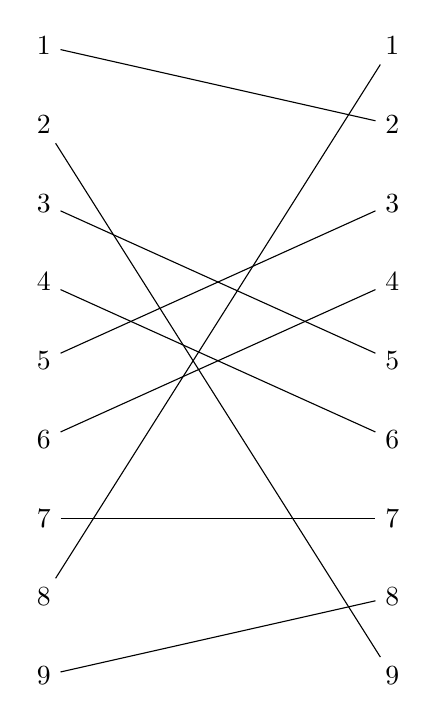
\begin{tikzpicture}
    % Definizione delle coordinate per la prima e la seconda colonna
    \foreach \i in {1,...,9} {
        \node[left]  (A\i) at (0, -\i) {\i};
        \node[right] (B\i) at (4, -\i) {\i};
    }
    % Collegamenti tra i numeri
    \draw (A1) -- (B2);
    \draw (A2) -- (B9);
    \draw (A3) -- (B5);
    \draw (A4) -- (B6);
    \draw (A5) -- (B3);
    \draw (A6) -- (B4);
    \draw (A7) -- (B7);
    \draw (A8) -- (B1);
    \draw (A9) -- (B8);
\end{tikzpicture}
\end{center}
\caption{Rappresentazione di una permutazione con diagramma ad arco.}
\label{fig:permutazione}
\end{figure}

Due permutazioni speciali sono la permutazione identità e l'n-ciclo. La prima non fa nulla, ovvero permuta ogni elemento in se stesso, la seconda permuta gli elementi in modo ciclico; ogni elemento viene permutato di una posizione a destra e l'ultimo va in prima posizione. 

$$
\epsilon \leftrightarrow
  \begin{pmatrix}
    1 & 2 & ... & n-1 & n \\
    1 & 2 & ... & n-1 & n
  \end{pmatrix}
$$

$$
  \begin{pmatrix}
    1 & 2 & ... & n-1 & n \\
    2 & 3 & ... & n & 1
  \end{pmatrix}
$$

\begin{definition}
    Date due permutazioni $\alpha, \beta$ la composizione (moltiplicazione) di esse restituisce una terza permutazione, applicando la seconda permutazione all'applicazione della prima su un elemento $k$ dell'insieme: 
$$
(\alpha \circ \beta)(k) = \beta(\alpha(k))), per \ k\in [n]
$$
\end{definition}
\begin{definition}
    Due permutazioni $\alpha,\beta$ sono dette inverse se $\alpha\beta=\epsilon$.
\end{definition}

Quest'ultima definizione è particolarmente importante perché permette di disfare una mossa del puzzle.

\begin{definition}
    Per ogni permutazione $\alpha$, esiste ed è unica una permutazione $\beta$ tale che $\alpha\beta = \beta\alpha = \epsilon$, in questo caso $\beta = \alpha^{-1}$. 
\end{definition}

Queste definizioni valgono anche per i prodotti (composizioni) di permutazioni: 
$$
(\alpha_1 \alpha_2...\alpha_k)^{-1} = \alpha_k^{-1}...\alpha_2^{-1}\alpha_1^{-1}
$$

\begin{definition}
L'insieme di tutte le permutazioni dell'insieme $[n]$ è detto gruppo simmetrico di grado $n$ ed è indicato con $S_n$. 
$$
S_n = \{\alpha | \alpha \ \acute{e} \ una \ permutazione \ di \ [n]\}
$$   
\end{definition}

Quando si parla di mosse di un puzzle spesso si usano le notazioni esponenziali, $\alpha^{-1}$ si indica con la permutazione inversa di $\alpha$, $\alpha^m$ vuol dire la permutazione $\alpha$ applicata $m$ volte.

\begin{definition}
    Per ogni $\alpha \in S_n$ esiste un intero positivo $m$ tale che $\alpha^m=\epsilon$, il minor $m$ tale che questa relazione valga è detto ordine di $\alpha$ e denotato con $ord(\alpha)$. 
\end{definition}

Tornando all'insieme $[n]\rightarrow \{1,2,3,...,9\}$ se $
\sigma = [\sigma(1),\sigma(2),...,\sigma(n)] = [2,9,5,6,3,4,7,1,8]
$ allora possiamo indicare tale permutazione con una notazione detta ciclica: 

\begin{figure}[h]
\begin{center}
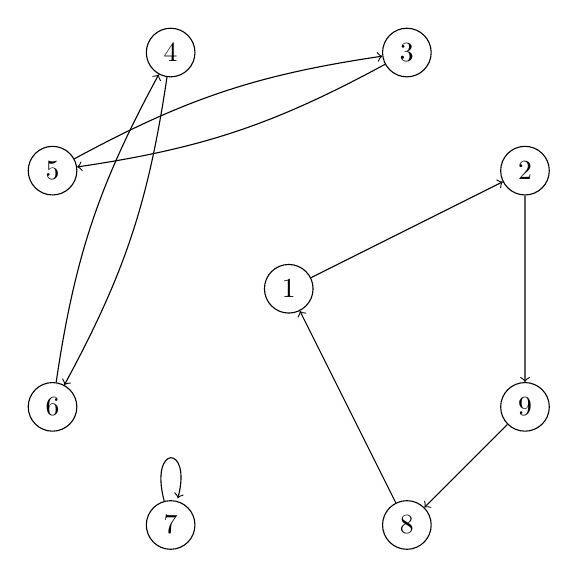
\begin{tikzpicture}[scale=1.5, every node/.style={draw, circle}, ->]
    % Definizione dei nodi in posizioni arbitrarie per un grafo
    \node (A1) at (0,0) {1};
    \node (A2) at (2,1) {2};
    \node (A3) at (1,2) {3};
    \node (A4) at (-1,2) {4};
    \node (A5) at (-2,1) {5};
    \node (A6) at (-2,-1) {6};
    \node (A7) at (-1,-2) {7};
    \node (A8) at (1,-2) {8};
    \node (A9) at (2,-1) {9};
    
    % Collegamenti tra i nodi con orientamento
    \draw[->] (A1) -- (A2);
    \draw[->] (A2) -- (A9);
    \path [->,bend left=10] (A3) edge (A5);
    \path [->,bend left=10] (A5) edge (A3);
    \path [->,bend left=10] (A4) edge (A6);
    \path [->,bend left=10] (A6) edge (A4);
    \draw[->] (A7) edge[loop above] (A7);
    \draw[->] (A8) -- (A1);
    \draw[->] (A9) -- (A8);
\end{tikzpicture}
\end{center}
\caption{Notazione ciclica.}
\label{fig:notCiclica}
\end{figure}


che si ottiene scrivendo gli elementi di ogni ciclo. 
Ad esempio nel caso descritto sopra definiamo: 
$$
(a_1,...,a_{l_1})(a_{l+1},...,a_{l_2})...() = (1,2,8,9)(3,5)(4,6)(7).
$$

Generalmente i cicli che contengono un solo elemento vengono ignorati, quindi ci rimane $(1,2,8,9)(3,5)(4,6)$.
Siccome una permutazione $(a_1,...,a_m)$ è detta m-ciclo, in questo caso la permutazione è il prodotto di un 4-ciclo e di due 2-cicli. 
Per definire la notazione ciclica di una permutazione partiamo dal valore minore, in questo caso $1$, scriviamo il numero in cui viene mappato, in questo caso $(1 \ 2)$ e continuiamo finchè non chiudiamo il ciclo $(1\ 2 \ 8\ 9)$.

Sia $\sigma=[\sigma(1), \sigma(2),...,\sigma(n)] \in S_n$. Un'inversione è un paio di indici $i\leq j$ tali che $\sigma(i)>\sigma(j)$. Indichiamo $Inv(\sigma)$ l'insieme delle inversioni e $inv(\sigma)$ il numero di inversioni. 

La fattorizzazione disgiunta di cicli è la fattorizzazione della permutazione in cicli nella notazione ciclica in cui nessun ciclo ha elementi in comune con un altro ciclo. 
Ad esempio se $f = (1,2,3)(4,5,6)\in S_6$ allora $f=gh$ con: 
$$
g=(1,2,3),f=(4,5,6).
$$
Questo è particolarmente importante in quanto ogni permutazione può essere scritta come prodotto di cicli disgiunti. Ad esempio una trasposizione è un 2-ciclo.

\begin{definition}
    Ogni permutazione in $S_n$ può essere espressa come prodotto di 2-cicli.
\label{2-cicli}
\end{definition}

Un k-ciclo $(a_1...a_{k-1}a_k)$, di dimensione $n$,  può essere scritto come prodotto di trasposizioni,  cioè $(a_1,...a_{k-1},a_{k}) = (a_1a_2)(a_1a_3)...(a_1a_{k-1})(a_1a_k)$.

\begin{proof}
    Data una qualsiasi permutazione $\alpha \in S_n$, tale permutazione può essere scritta come prodotto di cicli disgiunti $$\alpha = (a_1a_2...a_r)(b_1b_2...b_s)(c_1c_2...c_t)$$ e ogni ciclo può essere scomposto in un prodotto di due cicli seguendo la regola definita sopra (\ref{2-cicli}) $$\alpha = (a_1 a_2)(a_1 a_3)···(a_1 a_r)(b_1 b_2)(b_1 b_3)···(b_1 b_s)···(c_1 c_2)(c_1 c_3)···(c_1 c_t )$$
\end{proof}

Siccome ogni permutazione può essere generata da cicli disgiunti e ogni k-ciclo può essere generato da trasposizioni, le trasposizioni generano $S_n$. 
$$
(1,2)(2,3)(3,4) = (1,2,3,4)
$$

\subsection{Parità delle permutazioni ~\cite{8}}
Ogni permutazione $\alpha$ può essere rappresentata come il prodotto di un numero $k$ di 2-cicli. 
Il numero di 2-cicli che si utilizzano per rappresentare la permutazione definisce la sua parità.
Definiamo quindi due insiemi; l'insieme delle permutazioni pari $A_n$ e l'insieme delle permutazioni dispari $O_n$. Entrambi gli insiemi sono sottinsiemi dell'insieme di tutte le permutazioni $S_n$. 

\begin{theorem}
    Il numero di mosse per passare da una permutazione a un altra può variare ma la parità rimane uguale. 
\end{theorem}

Questo vuol dire che se $\alpha$ è una permutazione allora:
$$
\alpha=\tau_1\tau_2...\tau_r = \sigma_1\sigma_2...\sigma_s
$$
dove $\tau_i,\sigma_i$ sono 2-cicli e $r,s$ sono entrambi o pari o dispari. 

Ogni permutazione può essere rappresentata da un k-ciclo.
Ogni k-ciclo può essere rappresentato come il prodotto di $m-1$ trasposizioni (2-cicli).
Questo vuol dire che un $m$-ciclo è pari se $m$ è dispari ed è dispari se $m$ è pari. 
La correttezza di questo deriva da quanto definito sopra. (\ref{permutazioni})

Considerando la permutazione base $\pi_0=\{1,2,3\}$ e la permutazione finale $\pi=\{3,2,1\}$, rappresentabile volendo, come $(1,3)(2)$, si ottiene che la permutazione finale è ottenibile scambiando semplicemente il 3 con l'1, quindi con un numero dispari di mosse, oppure contando le dimensione dei cicli $|(1,3)|+|(2)|=3$ che è dispari. 
Si dice quindi che la permutazione $\pi$ è dispari. 
Si può, però, considerare di passare da $\pi_0$ a $\pi$ facendo prima uno scambio tra 2 e 1, poi uno scambio tra 2 e 3 e infine uno scambio tra 1 e 2. In questo caso si ottiene lo stesso risultato ma con 3 mosse. Si nota che il modo per arrivare al risultato è cambiato ma la parità della permutazione è rimasta la stessa.

Quindi se pensiamo a una trasposizione come ad una inversione, la parità di $\sigma$ dipende da $inv(\sigma)$

\begin{theorem}
    Ogni permutazione in $A_n$ può essere espressa come prodotto di 3-cicli.
\end{theorem}

Se $\alpha$ è una permutazione pari, infatti, significa che può essere scritta come prodotto di un numero pari di 2-cicli. Una volta fatto ciò basta raggruppare coppie adiacenti di trasposizioni ottenendo la permutazione sotto forma di prodotto di 3-cicli. 

\subsection{Esistenza o meno della soluzione ~\cite{8}}
L'idea di partenza del gioco è quella di iniziare da una disposizione casuale delle tessere e di riordinarle in modo da ottenere una disposizione voluta. 
Si possono, quindi, applicare le nozioni di permutazione per capire se il problema è risolvibile oppure no. 

Dato un insieme finito di valori $S_n=\{1,2,3,...,16\}$ e un piano di gioco iniziale, il quale può essere visto come una permutazione del piano di gioco con i numeri iniziali, ci interessa capire se tale permutazione è risolvibile. Ci interessa, quindi, sapere se esiste un numero finito di mosse che porta dalla permutazione del piano di gioco alla soluzione.

Data una disposizione iniziale delle pedine, che chiameremo $\sigma_0$, ciò che vogliamo capire è se dalla disposizione $\sigma_0$ si può arrivare alla disposizione $\sigma$, dove come $\sigma$ intendiamo la disposizione finale. 
Le permutazioni del piano di gioco $\sigma_0$ si possono dividere in due macrocategorie:
\begin{itemize}
    \item le disposizioni che fissano la casella vuota nella posizione 16;
    \item le disposizioni in cui la casella vuota non si trova in posizione 16;
\end{itemize}

Da questa distinzione derivano due teoremi su cui ci basiamo per parlare di risolvibilità del gioco del 15.

\begin{theorem}
    Una permutazione $\alpha$ del gioco del 15, che fissa il 16 è risolvibile se e solo se la permutazione $\alpha$ è una permutazione pari.
\end{theorem}

\begin{theorem}
    Una permutazione $\alpha$ del gioco del 15 che non fissa il 16 è risolvibile se e solo se la parità della permutazione coincide con la parità della distanza della pedina 16 dalla sua posizione obiettivo (cella 16).
\end{theorem}

Se rappresentiamo la disposizione finale delle tessere come:
$$\sigma=[1,2,3,4,5,6,7,8,9,10,11,12,13,14,15,16]$$ allora la disposizione iniziale può essere rappresentata, ad esempio, come: $$\sigma_0=[1,3,7,4,6,2,16,8,5,9,11,12,13,10,14,15]$$.

\begin{figure}[ht]
    \centering
    \begin{subfigure}{\textwidth}
        \centering
        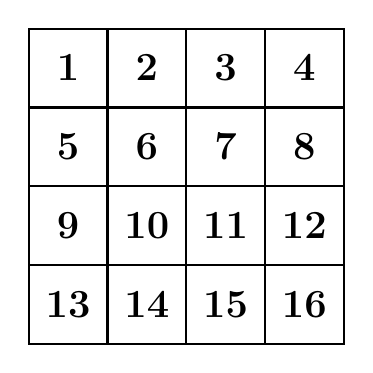
\begin{tikzpicture}
            \draw[thick] (0,0) rectangle (4,-4);
            \foreach \x in {1,2,3} \draw[thick] (\x,0) -- (\x,-4);
            \foreach \y in {1,2,3} \draw[thick] (0,-\y) -- (4,-\y);

            \foreach \y in {0,1,2,3} {
                \foreach \x in {0,1,2,3} {
                    \pgfmathtruncatemacro{\num}{\x + 4*\y + 1}
                    \ifnum\num<17
                        \node at (\x+0.5,-\y-0.5) {\textbf{\Large \num}};
                    \fi
                }
            }
        \end{tikzpicture}
        \caption{Disposizione finale (obiettivo) del gioco del 15.}
        \label{fig:dispFinale}
    \end{subfigure}

    \vspace{1em} % spazio verticale tra le due figure

    \begin{subfigure}{\textwidth}
        \centering
        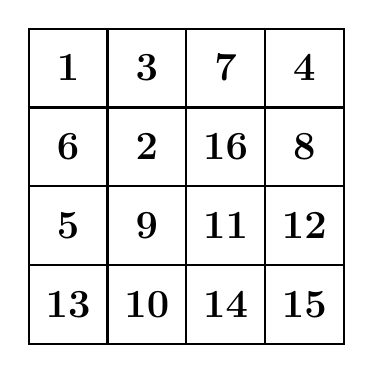
\begin{tikzpicture}
            \draw[thick] (0,0) rectangle (4,-4);
            \foreach \x in {1,2,3} \draw[thick] (\x,0) -- (\x,-4);
            \foreach \y in {1,2,3} \draw[thick] (0,-\y) -- (4,-\y);

            \node at (0.5,-0.5) {\textbf{\Large 1}};
            \node at (1.5,-0.5) {\textbf{\Large 3}};
            \node at (2.5,-0.5) {\textbf{\Large 7}};
            \node at (3.5,-0.5) {\textbf{\Large 4}};
            \node at (0.5,-1.5) {\textbf{\Large 6}};
            \node at (1.5,-1.5) {\textbf{\Large 2}};
            \node at (2.5,-1.5) {\textbf{\Large 16}};
            \node at (3.5,-1.5) {\textbf{\Large 8}};
            \node at (0.5,-2.5) {\textbf{\Large 5}};
            \node at (1.5,-2.5) {\textbf{\Large 9}};
            \node at (2.5,-2.5) {\textbf{\Large 11}};
            \node at (3.5,-2.5) {\textbf{\Large 12}};
            \node at (0.5,-3.5) {\textbf{\Large 13}};
            \node at (1.5,-3.5) {\textbf{\Large 10}};
            \node at (2.5,-3.5) {\textbf{\Large 14}};
            \node at (3.5,-3.5) {\textbf{\Large 15}};
        \end{tikzpicture}
        \caption{Disposizione iniziale del gioco del 15.}
        \label{fig:disposizioni}
    \end{subfigure}
\end{figure}

Per le proprietà descritte sopra (\ref{permutazioni}) un insieme di trasposizioni, l'insieme delle trasposizioni può variare ma non la sua parità.

Se il 16 è stato spostato di un numero dispari di celle, allora solo un insieme dispari di trasposizioni può portare a tale permutazione. 

\begin{figure}[h]
    \centering
        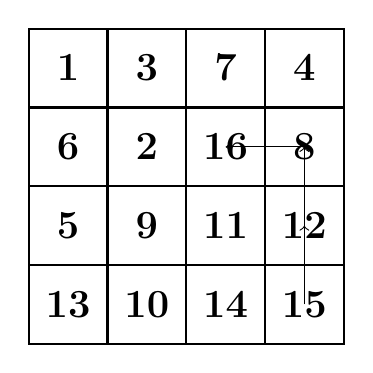
\begin{tikzpicture}
            % Disegna la griglia
            \draw[thick] (0,0) rectangle (4,-4);
            \foreach \x in {1,2,3} \draw[thick] (\x,0) -- (\x,-4);
            \foreach \y in {1,2,3} \draw[thick] (0,-\y) -- (4,-\y);
    
            % Inserisci i numeri in ordine
            \node at (0+0.5,-0-0.5) {\textbf{\Large 1}};
            \node at (1+0.5,-0-0.5) {\textbf{\Large 3}};
            \node at (2+0.5,-0-0.5) {\textbf{\Large 7}};
            \node at (3+0.5,-0-0.5) {\textbf{\Large 4}};
            \node at (0+0.5,-1-0.5) {\textbf{\Large 6}};
            \node at (1+0.5,-1-0.5) {\textbf{\Large 2}};
            \node at (2+0.5,-1-0.5) {\textbf{\Large 16}};
            \node at (3+0.5,-1-0.5) {\textbf{\Large 8}};
            \node at (0+0.5,-2-0.5) {\textbf{\Large 5}};
            \node at (1+0.5,-2-0.5) {\textbf{\Large 9}};
            \node at (2+0.5,-2-0.5) {\textbf{\Large 11}};
            \node at (3+0.5,-2-0.5) {\textbf{\Large 12}};
            \node at (0+0.5,-3-0.5) {\textbf{\Large 13}};
            \node at (1+0.5,-3-0.5) {\textbf{\Large 10}};
            \node at (2+0.5,-3-0.5) {\textbf{\Large 14}};
            \node at (3+0.5,-3-0.5) {\textbf{\Large 15}};
    
            \draw[->] (3+0.5,-3-0.5) -- (3+0.5,-2-0.5);
            \draw[->] (3+0.5,-2-0.5) -- (3+0.5,-1-0.5);
            \draw[->] (3+0.5,-1-0.5) -- (2+0.5,-1-0.5);
            
        \end{tikzpicture}
    \caption{Posizione della cella vuota rispetto alla posizione obiettivo.}
    \label{fig:notCiclica}
\end{figure}

Il primo passo consiste nel calcolare la parità del numero di spostamenti compiuti dalla casella vuota (il valore 16) per passare dalla posizione in $\sigma$ alla posizione in $\sigma_0$. Indichiamo tale distanza con $d(\sigma,\sigma_0)$, in questo $d(\sigma,\sigma_0)=3$ quindi è dispari.   

Rappresentiamo la disposizione $\sigma_0$ in notazione ciclica, ottenendo: $$(2,3,7,16,15,14,10,9,5,6)(1)(4)(8)(11)(12)(13)$$ eliminando i cicli singoli otteniamo un unico ciclo di 10 elementi. Siccome ogni ciclo di dimensione $n$ può essere scritto come prodotto di $n-1$ trasposizioni, possiamo andare a scriverla come prodotto di trasposizioni nel seguente modo:
$$
(2,3)(3,7)(7,16)(16,15)(15,14)(14,10)(10,9)(9,5)(5,6).
$$
Notiamo che sono in tutto 9 trasposizioni, quindi un numero dispari di scambi.

Abbiamo, quindi, dedotto che la disposizione $\sigma_0$ è stata ottenuta con un numero dispari di spostamenti della cella vuota.
Sappiamo, inolte, che la permutazione $\sigma_0$ può essere generata da un $k-$ciclo con $k$ dispari, dunque tale permutazione è dispari. 
Siccome tale permutazione può essere ottenuta con un insieme di trasposizioni, e siccome le due parità coincidono, otteniamo che la permutazione $\sigma$ è raggiungibile dalla permutazione $\sigma$ ergo il gioco ha soluzione. 

Un secondo metodo per calcolare la parità della permutazione consiste nel contare il numero di inversioni. 
Abbiamo già definito cosa si intende con inversione, nell'esempio rappresentato otteniamo un totale di 21 inversioni, cioè un valore dispari.
Questo metodo si presta meglio a una soluzione algoritmica. 

Consideriamo la disposizione sul piano di gioco come una permutazione delle celle che dove la cella contenente la pedina 16 è in posizione $z$, otteniamo: 
$$
a_1a_2a_3...a_{z-1}a_{z}a_{z+1}a_{15}
$$
Sia $N$ il numero di inversioni.
Sia $K$ l'indice della riga in cui si trova l'elemento vuoto. Definiamo il calcolo di $K$ come:
$$
K = \lfloor z/4 \rfloor + 1
$$

la soluzione, quindi, esiste se $K+N$ è pari, in quanto un numero pari può essere ottenuto come somma di due numeri pari o di due numeri dispari. In entrambi i casi si tratta di due numeri la cui parità coincide, che è ciò che vogliamo ottenere. 

\subsection{Algoritmo per il calcolo dell'esistenza o meno di una soluzione ~\cite{7}}

\begin{algorithm}[H]
\caption{Funzione per verificare se la disposizione del gioco del 15 ha soluzione}
\small  % Riduce la dimensione del font
\begin{algorithmic}[1]
\Require $a$: array di 16 valori che indicano le chiavi contenute nelle 16 posizioni del piano di gioco
\Function{esistenzaSoluzione}{$a$}
    \State $inv \gets 0$
    \For{$i \gets 0$ \textbf{to} $15$}
        \If{$a[i] \neq 0$}
            \For{$j \gets 0$ \textbf{to} $i-1$}
                \If{$a[j] > a[i]$}
                    \State $inv \gets inv + 1$
                \EndIf
            \EndFor
        \EndIf
    \EndFor
    \For{$i \gets 0$ \textbf{to} $15$}
        \If{$a[i] == 0$}
            \State $inv \gets inv + (1 + \lfloor i/4 \rfloor)$
        \EndIf
    \EndFor
    \If{$inv \mod 2 == 0$}
        \State \Return $1$
    \Else
        \State \Return $0$
    \EndIf
\EndFunction
\end{algorithmic}
\end{algorithm}

A causa del doppio ciclo for utilizzato per contare le inversioni, la complessità di tale algoritmo è di $O(n^2)$.

\section{Un primo approccio alla soluzione del puzzle}
Un primo approcio alla soluzione, dove con soluzione intendiamo un algoritmo capace di portare una disposizione del 15 alla disposizione finale, se la disposizione di partenza accetta soluzione, prevede di utilizzare gli algoritmi di ricerca.

Quello che possiamo fare è andare a spostare le pedine, passando da una configurazione a un'altra, seguendo un percorso dettato da qualche metrica che ci consenta di capire quando siamo più vicini alla soluzione.

Per farlo possiamo sfruttare degli algoritmi di ricerca sui grafi, vedendo il piano di gioco come un grafo e ogni nodo come una cella del piano. 

\subsection{Algoritmo A*}
Gli algoritmi di ricerca su grafi come \textit{Depth-First Search} (DFS), \textit{Breadth-First Search} (BFS) e \textit{best-first}, rappresentano approcci fondamentali alla risoluzione di problemi di esplorazione dello spazio degli stati. DFS esplora in profondità un cammino prima di tornare indietro, BFS visita i nodi per livelli, garantendo il ritrovamento del cammino più corto in grafi non pesati mentre best-first sceglie di espandere la ricerca verso il nodo più promettente, assegnando un punteggio a ciascun nodo \cite{15}. Mentre i primi due metodi risultano inefficaci in presenza di costi associati agli archi o quando si desidera ridurre lo spazio di ricerca con l'ausilio di informazioni euristiche, il metodo best-first diventa comodo per la soluzione del problema. 

In questo contesto si inserisce l'algoritmo A* (\textit{A-star}) \cite{15}, che combina la ricerca best-first con un meccanismo euristico per stimare il costo verso il nodo obiettivo. A* utilizza una funzione, per valutare il costo di una mossa, \( f(n) = g(n) + h(n) \), dove \( g(n) \) rappresenta il costo effettivo dal nodo iniziale al nodo \( n \), e \( h(n) \) è una funzione euristica che stima il costo minimo residuo da \( n \) al nodo obiettivo. Se l’euristica non sovrastima mai il costo reale, l’algoritmo A* trova un percorso ottimo.

Nel nostro caso andiamo a implementare l'algoritmo considerando:
\begin{itemize}
    \item $g(n)$: numero di mosse fatte finora;
    \item $h(n)$: distanza di Manhattan di una pedina da dove dovrebbe trovarsi;
\end{itemize}

\subsection{Ottimizzazione iniziale (conflitti lineari)}
Per ottimizzare l'algoritmo iniziale possiamo considerare il concetto di conflitto lineare. 

Un \textit{conflitto lineare} si verifica quando due tessere si trovano nella stessa riga (o colonna) della griglia, entrambe dovrebbero trovarsi in quella riga (o colonna) nella configurazione obiettivo, ma sono nell'ordine sbagliato rispetto alla destinazione finale. In questi casi, almeno una delle due tessere dovrà necessariamente essere spostata fuori dalla riga (o colonna) per permettere all’altra di raggiungere la propria posizione, causando un aumento delle mosse minime necessarie.

Possiamo utilizzare l'identificazione dei conflitti lineari per migliorare la funzione euristica di A*, aumentando la precisione rispetto alla semplice distanza di Manhattan. Quello che andiamo a fare è preferire le configurazioni che hanno meno conflitti lineari. 

\subsection{Algoritmo IDA* \cite{16}}
L'algoritmo IDA* (\textit{Iterative Deepening A*}) è una variante dell'algoritmo A* che ne conserva la funzione euristica ma utilizza meno memoria. A differenza di A*, che opera in modalità best-first, IDA* adotta un approccio basato su depth-first search (DFS), evitando così la memorizzazione dell'intero albero di ricerca. L'algoritmo esplora lo spazio degli stati iterativamente, imponendo a ogni iterazione un vincolo di soglia sul valore della funzione di valutazione \( f(n) = g(n) + h(n) \), dove \( g(n) \) rappresenta il costo del cammino dal nodo iniziale a \( n \) e \( h(n) \) una stima euristica del costo restante. Se durante una visita in profondità viene incontrato un nodo il cui valore di \( f \) supera la soglia corrente, esso viene scartato ma contribuisce all’aggiornamento della soglia per l’iterazione successiva. Questo meccanismo consente a IDA* di evitare percorsi ridondanti.

\section{Un possibile approcio a spanning-tree}
Considerando quando detto nell'introduzione, precisamente nel \cref{routing number}, possiamo pensare di andare a modellare il gioco del 15 a una soluzione che sfrutta il concetto di spanning-tree.

Cerchiamo quindi di trovare un modo per modellare l'approccio a "sottogruppi" al nostro contesto di lavoro. 

\subsection{Una prima idea}
L'idea è quella di trattare ogni pedina come una foglia dell'albero, portarla a destinazione effettuando solo scambi con la cella vuota e non muovere più tale pedina.

 Tuttavia, questo metodo si rivela inapplicabile a causa della forte interdipendenza tra le tessere. Ogni movimento della cella vuota coinvolge necessariamente lo spostamento di una tessera adiacente, il che implica che per collocare correttamente una pedina, è spesso necessario spostare temporaneamente altre tessere già posizionate.
 
 Inoltre, vincolare una tessera a restare ferma una volta posizionata impedisce l'esplorazione di configurazioni intermedie che sarebbero indispensabili per il completamento del puzzle. Di conseguenza, il problema non è risolvibile come una semplice sequenza indipendente di sottoproblemi locali: la soluzione richiede una pianificazione globale che tenga conto di vincoli combinatori e configurazioni transitorie.

\section{Dimostrazione}

\subsection{Modello algebrico del gioco}

Ogni configurazione del gioco del 15 può essere rappresentata da una permutazione dell'insieme $\{1, 2, \dots, 15\}$, che rappresenta le tessere numerate, più un simbolo aggiuntivo per la cella vuota (nel nostro caso il 16). I movimenti ammessi corrispondono a trasposizioni tra la cella vuota e una tessera adiacente. L'insieme delle configurazioni raggiungibili forma un sottogruppo $G$ del gruppo simmetrico $S_{16}$, il gruppo di tutte le permutazioni su 16 elementi. Più precisamente, il gruppo $G$ è generato dalle trasposizioni locali che coinvolgono il vuoto e una delle tessere vicine.

Poiché ogni mossa ammissibile coinvolge una sola tessera alla volta e il vuoto, le permutazioni ottenibili sono composte da cicli di lunghezza pari e dunque il gruppo risultante è contenuto nel gruppo alternante $A_{16}$ (il sottogruppo di permutazioni pari di $S_{16}$).

\subsection{Effetto della fissazione di tessere}
Quando si decide di ``fissare'' una tessera $t$ in una posizione specifica, si sta imponendo una restrizione alle permutazioni ammissibili: si considera solo il sottogruppo delle permutazioni che lasciano $t$ invariato. Se $G$ è il gruppo originale delle permutazioni raggiungibili, allora si considera il sottogruppo detto stabilizzatore:

\[
\text{Stab}_G(t) = \{ \pi \in G \mid \pi(t) = t \}
\]

Ogni nuova tessera fissata riduce ulteriormente lo spazio delle permutazioni consentite:

\[
\text{Stab}_G(t_1, t_2, \dots, t_k) = \{ \pi \in G \mid \pi(t_i) = t_i \text{ per ogni } i = 1, \dots, k \}
\]

Questa progressiva riduzione dello spazio delle permutazioni ha come effetto che pur essendo la configurazione finale ancora teoricamente raggiungibile nel gruppo $G$, essa non lo sia più nel sottogruppo stabilizzatore ottenuto fissando alcune tessere. In altri termini, il percorso verso la soluzione potrebbe richiedere mosse che temporaneamente ``sconvolgono'' le tessere già posizionate, per poi riposizionarle correttamente in seguito. L’approccio che impedisce tali mosse per principio elimina queste possibilità.

\section{Un possibile algoritmo risolutivo ~\cite{8}} 
Un possibile algoritmo risolutivo del gioco del 15 ha bisogno di un compromesso.
Risolvere il puzzle andando a considerare un processo che si divide in 2 fasi.

La prima fase consiste nel risolvere la prima riga da sinistra a destra:
\begin{itemize}
    \item è necessario trovare la pedina che si vuole portare nella posizione corretta della prima riga;
    \item se non è l'ultima pedina allora è necessario spostarla fino a raggiungere la posizione desiderata tenendo conto di:
    \begin{itemize}
        \item non è permesso spostare mai le pedine sistemate precedentemente;
        \item per spostare la pedina in una determinata posizione è necessario spostare le altre intorno ad essa finché non si è portata la cella vuota accanto ad essa; 
    \end{itemize}
    \item se l'ultima pedina non è in posizione, è necessario portarla nella posizione sotto a quella in cui deve andare. Eseguendo le seguenti mosse $\{$ sotto, sotto, destra, sopra, sinistra, sopra, destra, sotto, sotto, sinistra, sopra$\}$.
    \begin{figure}[h]
        \centering
        \includegraphics[width=0.8\linewidth]{movestoplace4.png}
        \caption{Mosse per portare il 4 in posizione}
        \label{fig:enter-label}
    \end{figure}
\end{itemize}
La seconda fase serve a concludere il gioco: 
\begin{itemize}
    \item ripeti la prima fase finché non sono rimaste solo due righe da sistemare; 
    \item ruota il piano di gioco di 45 gradi a destra;
    \item usa la fase uno per risolvere le nuove prime righe finché non sono rimaste solo due righe, ovvero finché non rimane un piano 2x2; 

    \begin{figure}[H]
        \centering
        \includegraphics[width=0.8\linewidth]{mosse45gradi.png}
        \caption{seconda fase}
        \label{fig:enter-label}
    \end{figure}
    \item sposta le caselle finché il vuoto e una delle altre 3 caselle non sono in posizione corretta, le altre due dovrebbero essere automaticamente sistemate;
\end{itemize}